\documentclass{standalone}
\usepackage{tikz}
\usepackage{../mss}
\usepackage{sansmath}

\usetikzlibrary{shapes.geometric,positioning,calc,petri,graphs,fit,backgrounds}
\tikzset{
        node distance=1.35cm and 1.35cm,
        >=latex,
        font=\sf\bfseries\sansmath,
        ,
        every edge/.append style={line width=1.0pt}
        textfeld/.style={align=center,minimum height=0.5cm,minimum width=1.5cm},
        pfeil/.style={->,line width=1.0pt},
        box/.style={rectangle,draw,line width=1.0pt,minimum height=1.5cm,minimum width=2.8cm,align=center},
        place/.style={circle,line width=1.0pt,draw=black,minimum size=6mm},
        transition/.style={rectangle,line width=1.0pt,draw=black,minimum size=6mm},
        module/.style={rectangle,fill=gray!25,line width=1.0pt,inner sep=10pt},
        module label/.style={text=gray!90},
        synchronization/.style={draw,dashed,rounded corners,inner sep=6pt}
        }

\tikzgraphsset{
    every graph/.style = {use existing nodes}
}

\begin{document}
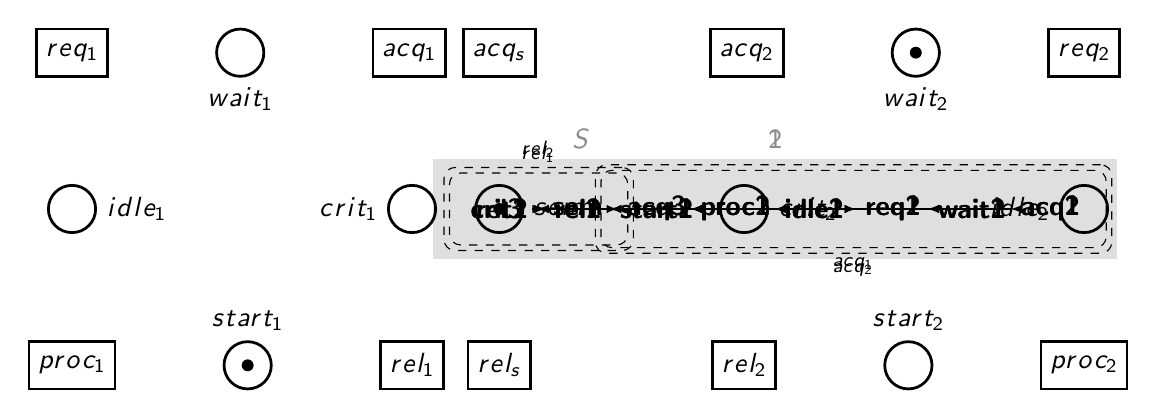
\begin{tikzpicture}
    % semaphor
    \node[place,tokens=1,label=right:$ sem $] (sem) {};
    \node[transition] (acq3) [above=of sem] {$ acq_s $};
    \node[transition] (rel3) [below=of sem] {$ rel_s $};
    \graph{rel3 -> sem -> acq3};

    % process 1 on the left
    \node[place,label=left:$ crit_1 $] (crit1) [left=of sem] {};
    \node[transition] (rel1) [below=of crit1] {$ rel_1 $};
    \node[place,tokens=1,label=above:$ start_1 $] (start1) [left=of rel1] {};
    \node[transition] (proc1) [left=of start1] {$ proc_1 $};
    \node[place,label=right:$ idle_1 $] (idle1) [above= of proc1] {};
    \node[transition] (req1) [above=of idle1] {$ req_1 $};
    \node[place,label=below:$ wait_1 $] (wait1)  [right=of req1] {};
    \node[transition] (acq1) [right=of wait1]{$ acq_1 $};
    \graph{crit1 -> rel1 -> start1 -> proc1 -> idle1 -> req1 -> wait1 -> acq1 -> crit1};


    % process 2 on the right
    \node[place,label=right:$ crit_2 $] (crit2) [right=of sem] {};
    \node[transition] (rel2) [below=of crit2] {$ rel_2 $};
    \node[place,label=above:$ start_2 $] (start2) [right=of rel2] {};
    \node[transition] (proc2) [right=of start2] {$ proc_2 $};
    \node[place,label=left:$ idle_2 $] (idle2) [above= of proc2] {};
    \node[transition] (req2) [above=of idle2] {$ req_2 $};
    \node[place,tokens=1,label=below:$ wait_2 $] (wait2)  [left=of req2] {};
    \node[transition] (acq2) [left=of wait2]{$ acq_2 $};
    \graph{crit2 -> rel2 -> start2 -> proc2 -> idle2 -> req2 -> wait2 -> acq2 -> crit2};

    % synchronizations
    \node[synchronization,
        fit=(acq1)(acq3),
        label={below:$ \synchronization_{acq_1} $}
    ]{};
    \node[synchronization,
        fit=(rel1)(rel3),
        label={above:$ \synchronization_{rel_1} $}
    ]{};
    \node[synchronization,
        fit=(acq2)(acq3),
        inner sep=8pt,
        label={below:$ \synchronization_{acq_2} $}
    ]{};
    \node[synchronization,
        fit=(rel2)(rel3),
        inner sep=8pt,
        label={above:$ \synchronization_{rel_2} $}
    ]{};

    % modules
    \begin{scope}[on background layer]

        \node[module,
            fit=(crit1)(rel1)(start1)(proc1)(req1)(acq1),
            label={[module label]above:$ \module{1} $}
        ] {};
        \node[module,
            fit=(sem)(rel3)(acq3),
            label={[module label]above:$ \module{S} $}
        ] {};
        \node[module,
            fit=(crit2)(rel2)(start2)(proc2)(req2)(acq2),
            label={[module label]above:$ \module{2} $}
        ]{};
    \end{scope}

\end{tikzpicture}
\end{document}